\documentclass[10pt]{article}
\usepackage[T1]{fontenc}
\usepackage[utf8]{inputenc}
\usepackage[margin=0.85in]{geometry}
\usepackage{amsmath}
\usepackage{booktabs}
\usepackage{array}
\usepackage{graphicx}
\usepackage{float}
\usepackage{placeins}
\usepackage{tabularx}
\usepackage{hyperref}
\hypersetup{colorlinks=true,linkcolor=blue!50!black,citecolor=blue!50!black,urlcolor=blue!50!black}
\usepackage{xcolor}
\graphicspath{{figures/}}

\title{New Trace Features, Feature Tiers and Learned Importance:\\ Results of 2026-10-21}
\author{ML-assisted optimization of CCD operating parameters --- working note}
\date{21 October 2026}
\newcommand{\code}[1]{\texttt{#1}}
\newcommand{\se}{\sigma_e}
\emergencystretch=3em
\newcolumntype{L}{>{\raggedright\arraybackslash}X}

\begin{document}
\maketitle

\begin{abstract}
Fifty-six new scalar trace features and four new curves were added to \code{src/trace\_features.py}. Forty-nine come from
signal analysis in other fields: radar, finance, electrophysiology, gravitational-wave detectors, cardiology, astronomy,
audio, machine diagnostics, metrology and seismology. They were tested on the 59 usable board-101 traces of the
2026-10-12 packet tests. Two families stand out. The \emph{start-of-pixel} features are the only new ones that separate
the settings (best: settings $F = 264$, repeat share 0.02). The \emph{telegraph and jump} features single out ch2, whose
excess noise is a Gaussian part plus discrete steps that an ordinary $\sigma$ cannot separate. A third family, the
\emph{clocking-region} features (the vertical-clock block before a row and the first horizontal block after it), was
added at the end of the day; all four of its main features land in the top evidence tier. So does the depth of a
sharp dip just before the per-cycle pulse, which is fixed by the amplifier.

With 141 scalar features, not every model can take them all. A synthetic tolerance test shows that the plain Gaussian
process collapses with only 20 uninformative columns ($\se$ error $+51$ percentage points), while trees are immune. The
features are therefore sorted into tiers: an implementation tier (where a feature came from), an evidence tier A1/A2/B/C
(what the data say, no labels needed) and a per-model feature set. The training script can now select tiers
(\code{--feature-tiers}), compare them (\code{--tier-ablation}), and feed every model more and more features in
label-free orders (\code{--feature-ladder}). Because the label-free tiers can demote the most direct noise estimators,
a protected set of eight physical estimators is now given to every model. Finally, a learned importance method
(stability selection and permutation importance against shadow features) was built and checked on five synthetic
datasets: 1 of 100 added noise columns reached its top tier L1, on the smallest (13-packet) dataset.
\end{abstract}

\tableofcontents

%======================================================================
\section{Summary}

\begin{itemize}
  \item \textbf{The first-skip offset is a baseline slope.} The CDS of the first skips of every pixel reads the slope of a
        decaying baseline. Regressing the offset on the in-window slope gives a lever arm of $-212$ samples, against the
        $-207$-sample spacing of the window centres ($R^2 = 0.97$). Its size rises by 21\,\% only when all horizontal
        low rails are lowered: horizontal-clock feedthrough.
  \item \textbf{The start-of-pixel group separates settings.} The matched-filter transient amplitude has settings
        $F = 264$, amplifier $F = 70$ and repeat share 0.02. No noise feature, old or new, separates these four
        settings, because they did not change the noise.
  \item \textbf{ch2 has random telegraph switching.} Steps appear inside single integration windows in 8.2\,\% of ch2's
        windows and in none of the others. The jumps carry 27--28\,\% of ch2's CDS variance; its rms is 22.5\,ADU,
        but the jump-robust sigma is 16.8\,ADU.
  \item \textbf{No dominant pickup waveform on the good amplifiers.} On ch0 the three largest waveform modes of the skip
        cycles carry only 0.9\,\% of the CDS variance and 106 modes are needed for 90\,\% (medians over traces: 69--105
        modes on ch0, ch1, ch3). On ch2 only about 8 modes carry 90\,\%: its excess noise sits in a few large modes.
  \item \textbf{The clocking regions carry setting information.} The V-transfer peak-to-peak (settings $F = 544$), the
        H/V peak-to-peak ratio ($F = 879$), the level slope in the V block before row 2 ($F = 45$, steeper with the V
        rails low) and the settling at the start of the first H burst after the V clocking ($F \approx 1.3\times10^4$, largest with the H rails low)
        are all repeatable (repeat share $\le 0.03$) and not redundant with any existing feature. The steep climb in
        the first V block is real but not repeatable: the trace starts at a random point in that block.
  \item \textbf{The dip before the pulse is an amplifier fingerprint.} A dip 120--130\,ns before the per-cycle pulse is
        $-505$ to $-990$\,ADU deep depending on the amplifier, with repeat share 0.001, and does not change with any of
        these settings (none touched RG, SW, OG or DG).
  \item \textbf{Tiers.} 141 scalar features: evidence tiers A1 37, A2 36, B 33, C 35, plus the protected set P (8).
        The plain GP gets P only; trees can take everything.
  \item \textbf{Guarding the tiers.} The label-free tiers put the most direct $\se$ estimator and the kTC noise in B. A
        protected set P of eight physical estimators now goes to every model; on synthetic data this alone took the
        plain GP from collapsed to 9.6\,\% ($\se$) and 0.9\,\% (gain). Features are never ordered by the labels.
  \item \textbf{Feature ladder.} On synthetic data the plain GP is best with 8--15 features and collapses beyond;
        \code{gp\_dim} stays flat up to all features; \code{gp\_saas} loses $\lambda$ with more features; nn degrades with
        every added step, ridge is best near 25--45, trees are flat.
  \item \textbf{Learned tiers.} L1 (both methods confirm, by a margin) contained 1 of 100 noise columns over five
        synthetic datasets (on the 13-packet one). L2 (a candidate) contained 3--6 of 20 noise columns, so it is a list
        to look at, not a feature set. The learned tiers are diagnostics only.
\end{itemize}

%======================================================================
\section{The new features and where they came from}
\label{sec:features}

Two literature searches looked for hand-computable features in other fields: \code{signal\_analysis\_features.md}
(21 fields, 49 candidates) and \code{landscape\_exploratory.md}, both in \code{docs/literature/}. Each candidate was piloted on real traces
before it was implemented. The new code is \code{src/trace\_features\_extra.py}; 19 unit tests with known answers are in
\code{tests/test\_trace\_features\_new.py}. Computing all features takes about 1.2\,s per trace.

\begin{table}[H]
\centering\small
\begin{tabularx}{\textwidth}{>{\raggedright\arraybackslash}p{4.4cm}>{\raggedright\arraybackslash}p{3.2cm}L}
\toprule
feature(s) & field & the idea \\
\midrule
start: transient amplitude, matched filter & radar and sonar & project each pixel onto the trace's own mean transient; about 30\,\% less noise than reading skip 0 \\
start: in-cycle slope at skip 0 & chromatography (derivative filters), CDS theory & the baseline slope inside the window \\
start: first-skip excess per volt H & our own \code{edge: dip per volt} & divide by the H-clock swing so settings compare \\
noise: waveform modes for 90\,\% of the CDS variance & cardiology (KLT of heartbeats), machine diagnostics & treat the 5000 skip cycles like heartbeats, split them into modes and give each mode's exact share of the CDS variance \\
noise: null-CDS noise, kurtosis, lag-1 autocorrelation & gravitational-wave detectors (null streams), metrology (A--A tests) & a CDS between the two halves of the pedestal window, where no charge moves \\
discrete: in-window step rate and amplitude & electrophysiology (single-channel patch clamp), changepoint statistics & detect open/closed steps; here, telegraph steps of a trap \\
noise: jump-robust CDS sigma, discrete: jump share & high-frequency finance (MedRV) & separate the smooth noise from the jumps \cite{ads2012} \\
discrete: jump count (Lee--Mykland) & finance & a jump test against a local volatility estimate \cite{lm2008}; nominally at 1\,\%; after correcting a missing constant (2026-10-22) it still flags about 0.26 jumps per pure-Gaussian 490-skip series with 20-skip windows, so it is a relative count \\
noise: structure-function excess & astronomy (light curves) & the time scale of the noise inside the window \\
noise: CDS spectral centroid & audio and speech & the mean frequency of the spectrum \\
discrete: crest factor & machine-vibration diagnostics & peak over rms \\
noise: Hadamard and modified Allan deviation & time and frequency metrology & drift-insensitive versions of the Allan deviation \cite{riley2008} \\
discrete: STA/LTA maximum & seismology & short- over long-term average, the earthquake trigger \\
discrete: line count, frequency, phase coherence & oceanography (multitaper F-test), gravitational waves & pickup lines with a stated false-alarm rate \cite{thomson1982} \\
clock: V-block slope, V and H/V peak-to-peak, first H block of a row & our own trace inspection & what the clock feedthrough and the output level do during the transfers (Section~\ref{sec:clock}) \\
\bottomrule
\end{tabularx}
\caption{The most useful new features and the field each came from.}
\label{tab:fields}
\end{table}

The start-of-pixel group did not come from another field: it grew out of the question whether the first-skip offset is
worth studying. The pilot found that it is a baseline slope, and the group measures it.

\paragraph{What did not carry over.} The pickup-line features are real but change from trace to trace, so they are in
tier C for now. Heart-rate-variability measures (RMSSD, Poincar\'e SD1/SD2) are exact functions of the lag-1
autocorrelation and were not implemented; spectral flatness was redundant and left out. DFA, the sample and permutation
entropies and the red-noise $\beta$ looked weak in the pilots but were implemented as tier 2: the entropies separate the
amplifiers (tier A2), DFA is unstable (tier C) and $\beta$ is moderate (B). Also left out: hidden-Markov dwell times, step rise times, jitter decomposition, spectral flux and cepstrum.

\paragraph{The full list.} By implementation tier (Section~\ref{sec:tiers}):
\begin{itemize}
  \item \textbf{Tier 1} (29 scalars, 2 curves): start-of-pixel lever arm, slope-explained fraction, in-cycle slope,
        time constant, amplitude, excess per volt H; slope-corrected CDS rise; null-CDS noise and kurtosis; in-window
        step rate and amplitude; jump-robust sigma and jump share; 1/f corner and exponent; Hadamard deviation;
        waveform-mode share and count; line count, frequency, amplitude and two phase coherences. Curves: the mean
        start transient and the Hadamard deviation. Clocking regions: V-block level slope, V-transfer
        peak-to-peak, H/V peak-to-peak ratio, first-H-block excess. Pre-pulse dip depth and dip/pulse ratio.
  \item \textbf{Tier 2} (27 scalars, 2 curves): row-start/inner ratio, reset jump, mode frequency and damping, fast
        decay, matched-filter amplitude, ringing frequency; null-CDS autocorrelation; Lee--Mykland count, STA/LTA,
        crest factor, volatility clustering, whitened kurtosis, spectral kurtosis; Lorentzian corner; structure-function
        excess; lag-1 autocorrelation of 10-skip means, DFA, spectral slope and centroid, sample and permutation
        entropy, red-noise $\beta$; whole-trace line frequency; common-pattern spread; baseline--CDS correlation; the
        level slope of the leading V block.
        Curves: the within-cycle structure function and the modified Allan deviation.
\end{itemize}

%======================================================================
\section{Results on the 59 real traces of 2026-10-12}
\label{sec:real}

\paragraph{Data.} Board 101: 5 settings (reference, VDD $-20.5$\,V, vertical low rails and TG, all horizontal low rails,
H3\_A\_L only) $\times$ 3 repeats $\times$ 4 amplifiers, less one damaged ch3 trace.

\paragraph{Measures.} \emph{Settings F} is the one-way ANOVA $F$ over the four changed settings (all taken with NCOLPRE 185,
so the reference's different NCOLPRE cannot fake a separation), per amplifier ch0, ch1, ch3; the minimum is reported.
\emph{Amplifier F} is the ANOVA $F$ over the four amplifiers within each setting; the median is reported. With df $(3, 8)$,
$F > 4$ means $p < 0.05$. The \emph{repeat share} is the within-(setting, amplifier) variance over the total: 0 is
perfectly repeatable, about 1 is pure repeat noise.

\begin{figure}[H]
\centering
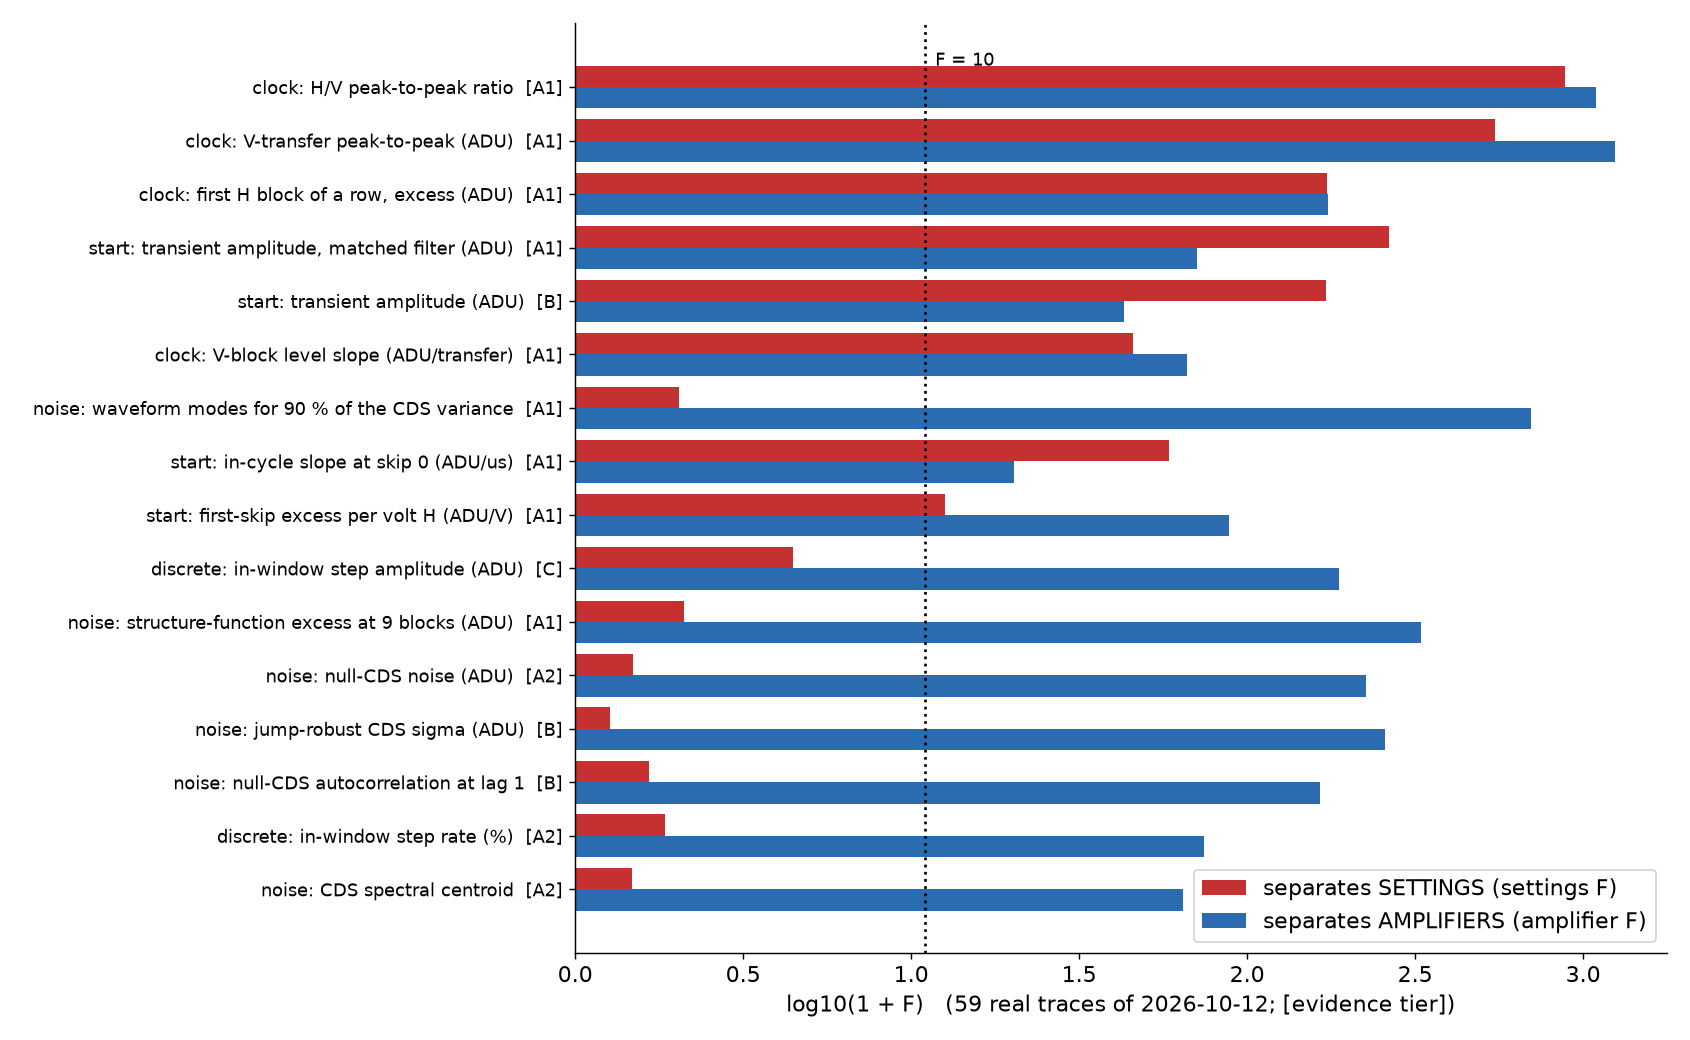
\includegraphics[width=\textwidth]{fig_top_new_features.png}
\caption{The 16 most informative new features. Red: separation of the settings. Blue: separation of the amplifiers.
The evidence tier is in brackets. Only the start-of-pixel features separate settings.}
\label{fig:top}
\end{figure}

\subsection{The start-of-pixel transient}

\begin{figure}[H]
\centering
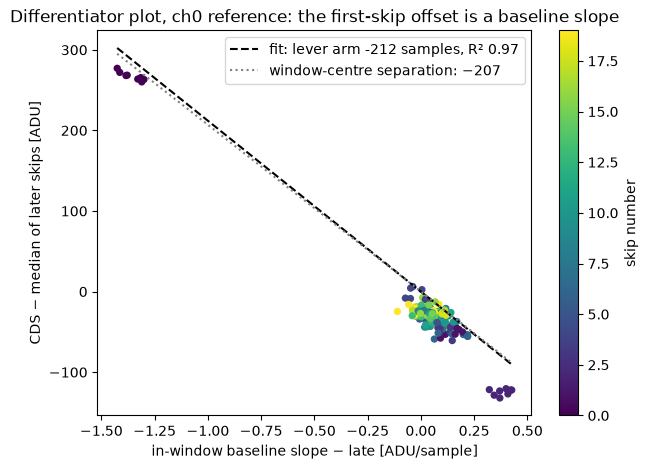
\includegraphics[width=0.52\textwidth]{nb_differentiator.png}\hfill
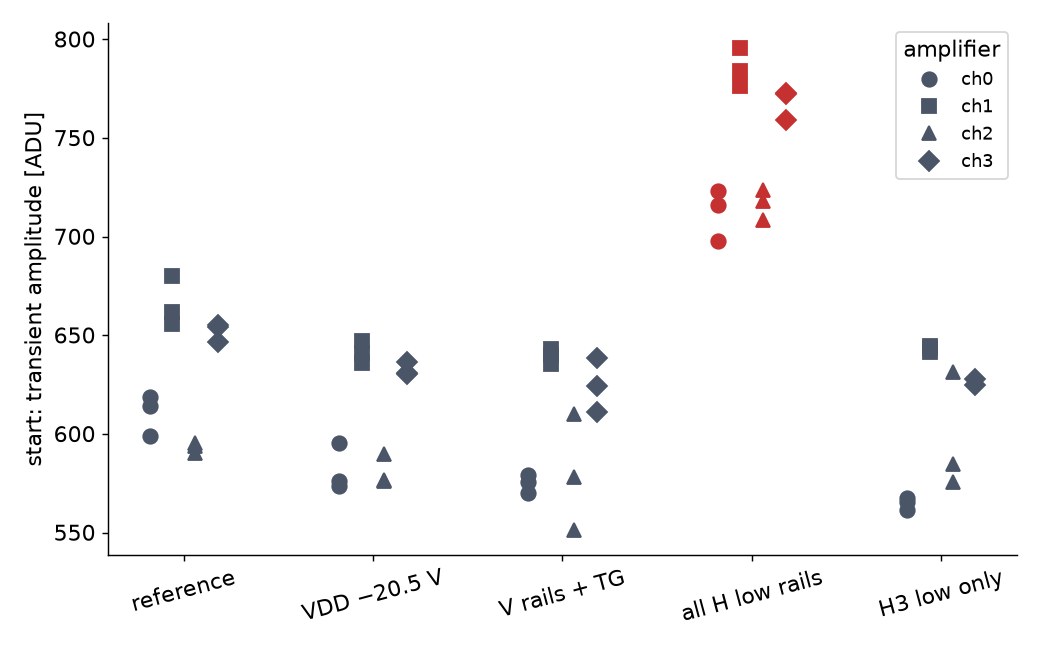
\includegraphics[width=0.46\textwidth]{fig_start_amplitude.png}
\caption{Left: the first-skip offset against the in-window baseline slope (ch0, reference). The fitted lever arm,
$-212$ samples, matches the $-207$-sample spacing of the window centres: the CDS reads a slope. Right: the transient
amplitude moves only when all horizontal low rails are lowered (red), on all four amplifiers.}
\label{fig:start}
\end{figure}

The first skips of every pixel carry about $+250$ to $+290$\,ADU at skip 0 (median per amplifier). Inside skip 0 the baseline decays as an exponential with
$\tau \approx 12\,\mu$s. The amplitude is about 615\,ADU at the other settings and 741\,ADU with all horizontal low rails
lowered (+21\,\%); lowering H3 alone does not move it.

\begin{table}[H]
\centering\small
\begin{tabular}{lcccc}
\toprule
feature & settings $F$ min & amplifier $F$ & repeat share & tier \\
\midrule
start: transient amplitude, matched filter & 264 & 70 & 0.02 & A1 \\
start: transient amplitude & 171 & 42 & 0.04 & B (same cluster) \\
start: in-cycle slope at skip 0 & 58 & 19 & 0.07 & A1 \\
start: first-skip excess per volt H & 12 & 87 & 0.04 & A1 \\
start: slope-explained fraction & 2.4 & 12 & 0.17 & A2 \\
start: CDS-slope lever arm & 1.0 & 14 & 0.20 & A2 \\
start: reset jump skip 0 to 1 & 0.7 & 26 & 0.14 & A2 \\
start: transient time constant & 1.9 & 2.1 & 0.58 & C (unstable) \\
\bottomrule
\end{tabular}
\caption{The start-of-pixel group.}
\end{table}

\subsection{Telegraph switching and jumps on ch2}

\begin{figure}[H]
\centering
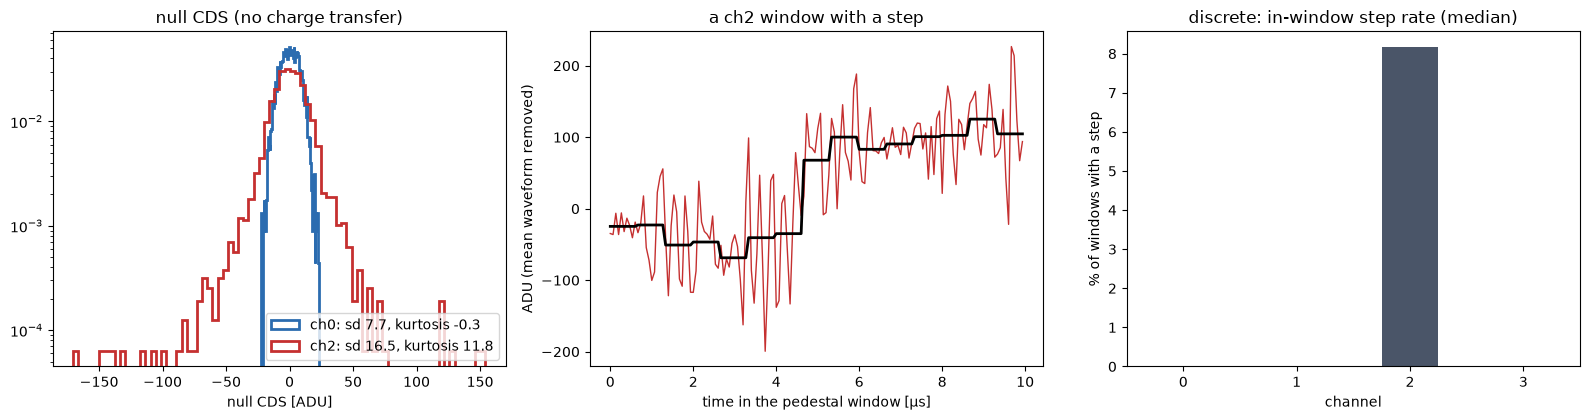
\includegraphics[width=\textwidth]{nb_null_cds.png}
\caption{Left: the null CDS (no charge transfer) of ch0 and ch2. Middle: a ch2 window with a telegraph step. Right: the
in-window step rate per amplifier.}
\label{fig:null}
\end{figure}

\begin{figure}[H]
\centering
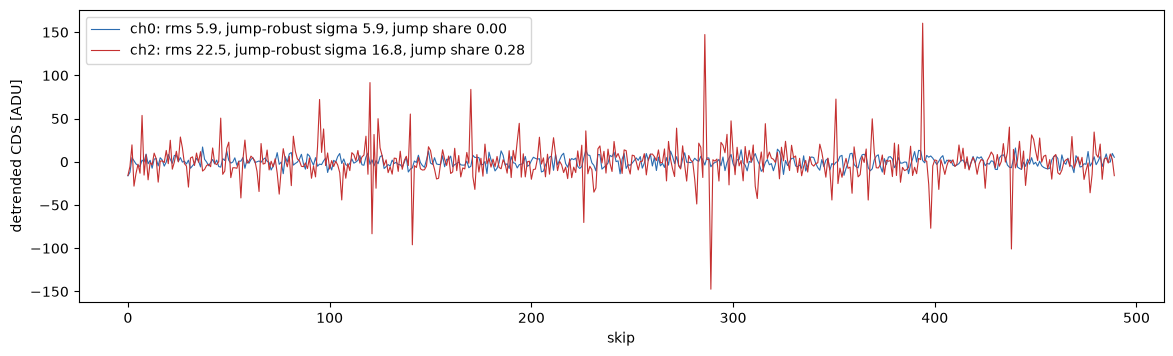
\includegraphics[width=\textwidth]{nb_jumps.png}
\caption{The CDS along the skips, ch0 and ch2. The jumps carry 28\,\% of ch2's CDS variance.}
\label{fig:jumps}
\end{figure}

\begin{table}[H]
\centering\small
\begin{tabular}{lccccc}
\toprule
feature (median per amplifier) & ch0 & ch1 & ch2 & ch3 & amplifier $F$ \\
\midrule
discrete: in-window step rate (\%) & 0 & 0 & \textbf{8.2} & 0 & 73 \\
discrete: null-CDS kurtosis & $-0.34$ & $-0.20$ & \textbf{5.2} & $-0.11$ & 49 \\
discrete: jump share of CDS variance & 0.001 & 0.005 & \textbf{0.27} & 0.005 & 32 \\
noise: null-CDS noise (ADU) & 7.8 & 7.1 & \textbf{20.4} & 8.0 & 225 \\
\bottomrule
\end{tabular}
\caption{The telegraph and jump features. The steps are $\pm 40$--110\,ADU, equally often up and down, inside one
10\,$\mu$s window with no charge transfer: random telegraph switching in the output stage.}
\end{table}

This matters for $\se$. An ordinary $\sigma$ of the CDS mixes the Gaussian noise with the jumps. The jump-robust sigma
(from MedRV, the median realized variance \cite{ads2012}) and the jump share separate the two.

\subsection{The noise budget}

\begin{figure}[H]
\centering
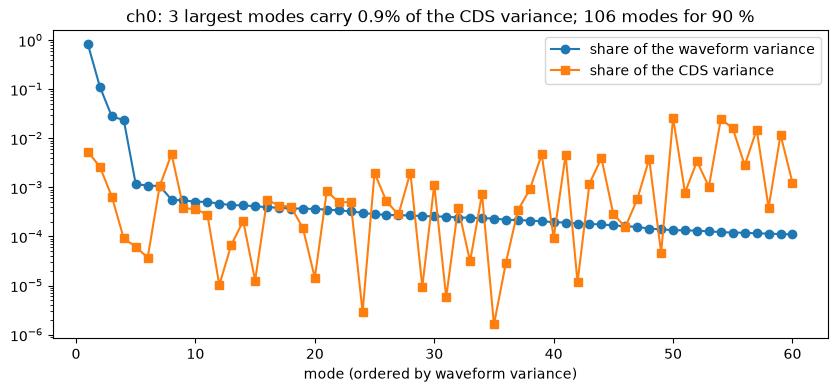
\includegraphics[width=0.85\textwidth]{nb_noise_budget.png}
\caption{The noise budget: the residual skip cycles split into waveform modes (principal components), and each mode's
exact share of the CDS variance (ch0, reference). The three largest modes carry 0.9\,\% of it; 106 modes are needed for 90\,\%.}
\label{fig:budget}
\end{figure}

The large clock and reset fluctuations of the waveform do not reach the CDS, because the CDS weights cancel them. There
is no single pickup waveform to subtract on the good amplifiers (69--105 modes for 90\,\%, medians over traces). ch2 is
the exception: about 8 modes carry 90\,\% of its CDS variance. The number of modes needed for 90\,\% therefore separates
the amplifiers very well (amplifier $F \approx 700$).

\subsection{Other noise-shape features}

The Hadamard and modified Allan deviations (Figure~\ref{fig:allan}), the sample entropy, the spectral slope and centroid,
the crest factor, the whitened kurtosis, the Lee--Mykland count, STA/LTA and the permutation entropy all separate the
amplifiers ($F$ 12--700) but not these settings. Unstable for now (repeat share 0.6--1.3): the pickup-line features, the
start-transient modes, the transient time constant, the 1/f and Lorentzian corners, and volatility clustering. The 1/f
features need longer time scales than a 0.2\,s trace offers; the delayInt scan should change that.

\begin{figure}[H]
\centering
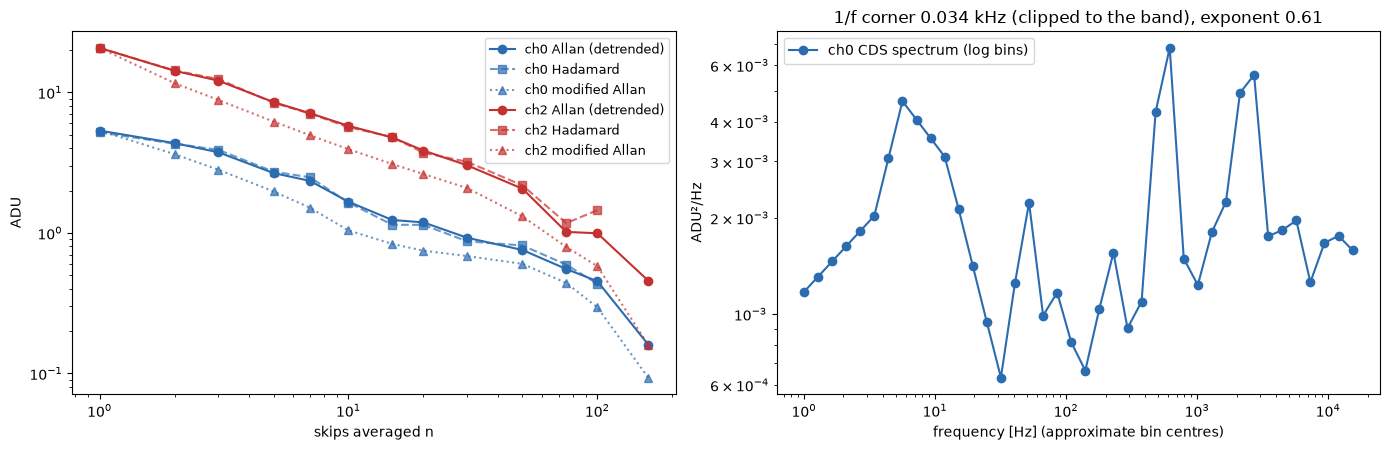
\includegraphics[width=0.8\textwidth]{nb_allan.png}
\caption{Allan, Hadamard and modified Allan deviations of the CDS.}
\label{fig:allan}
\end{figure}

\subsection{The clocking regions}
\label{sec:clock}

Between the pixels the trace records the clocking itself: a block of 20 vertical transfers before every row, and 20
horizontal transfers before every pixel (3720 for the prescan of a row with NCOLPRE 185). Three things stand out by eye:
the first V block climbs steeply while the second is nearly flat; the H and V transfers have very different sizes; and
the first H block after coming off a row looks different from the others (Figure~\ref{fig:clock}). A pilot
(\code{lvl1/feature\_study/clock\_pilot/}) measured them on the 59 traces, and the best became the \code{clock:} group.

\begin{figure}[H]
\centering
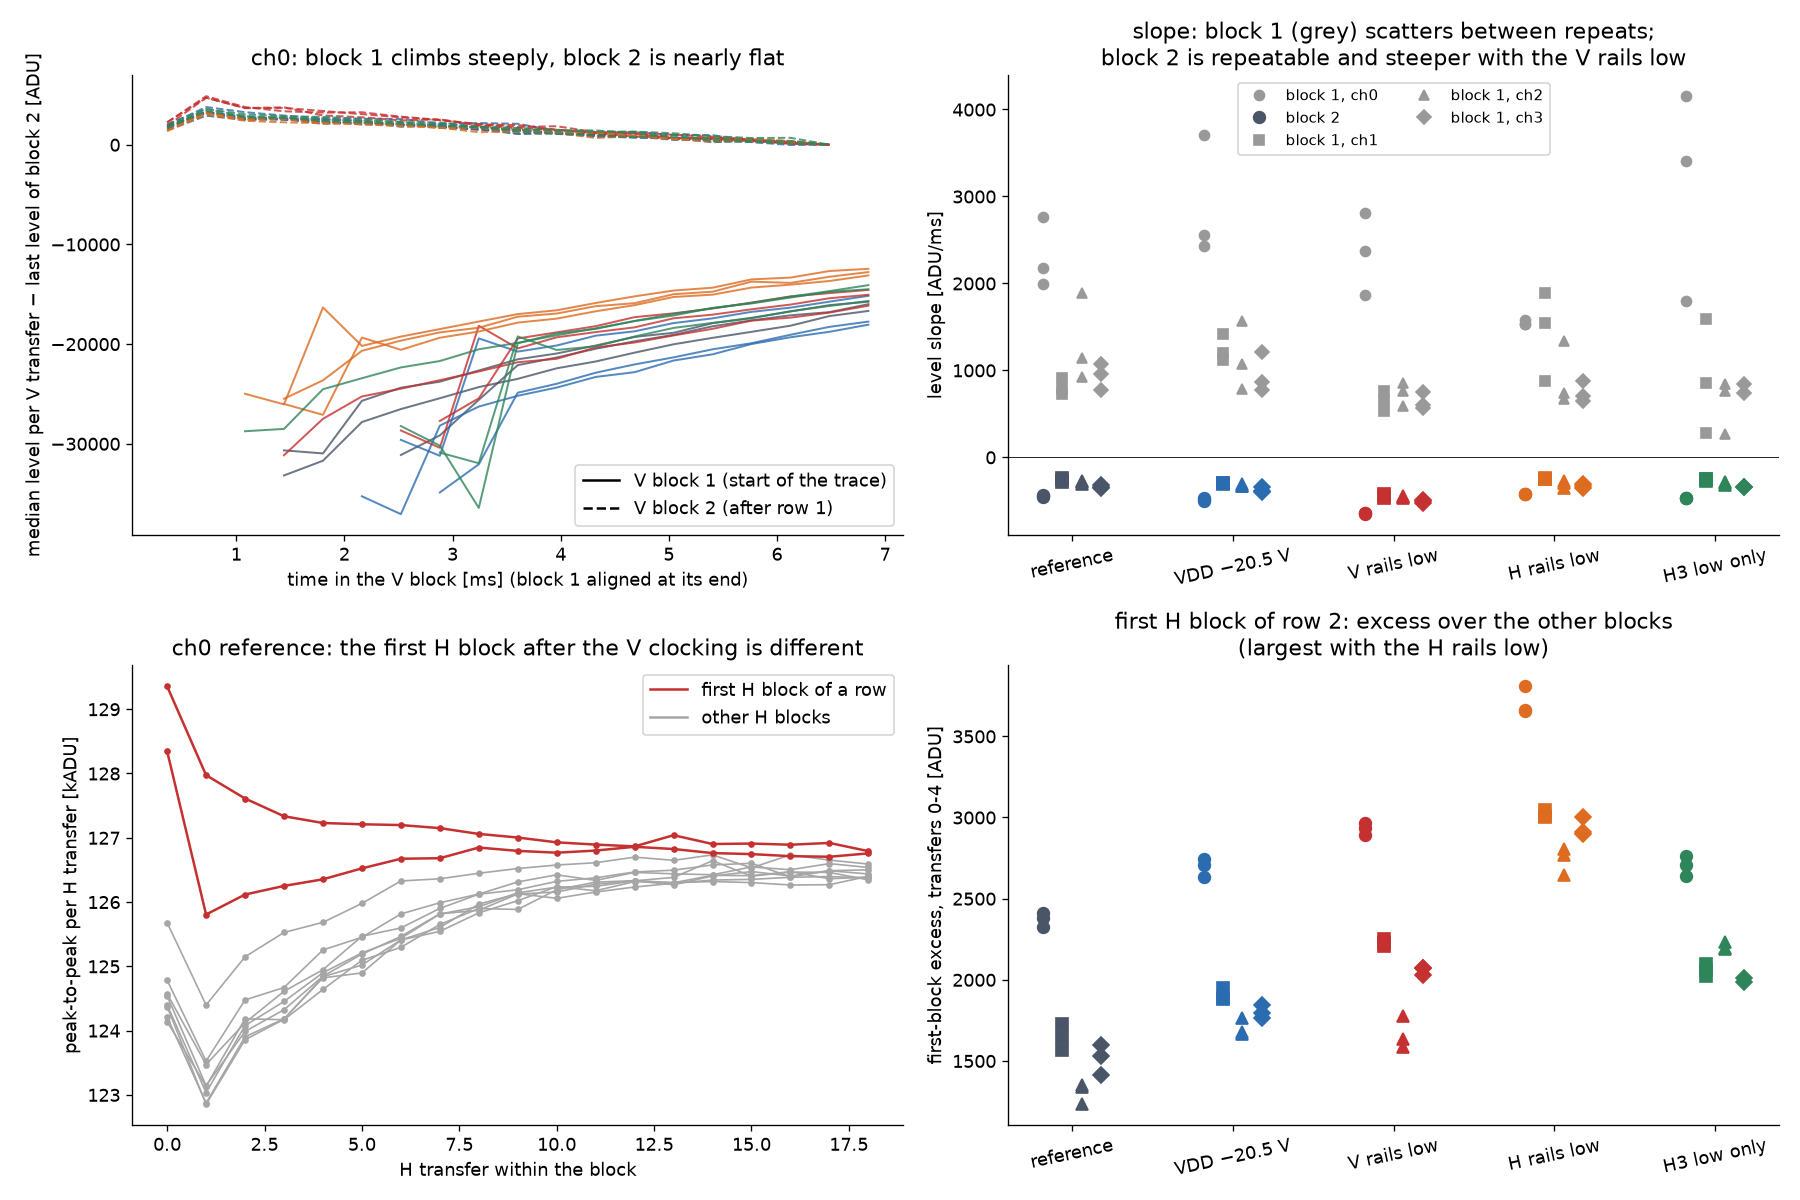
\includegraphics[width=\textwidth]{fig_clock_regions.png}
\caption{Top left: median level per V transfer, ch0, for the leading block (solid, aligned at its end) and the block
before row 2 (dashed). Top right: the two level slopes per setting; the leading block (grey) scatters, the second is
repeatable. Bottom left: peak-to-peak per H transfer within each H block, ch0 reference; red are the first blocks of a
row. Bottom right: the excess of the first H block of row 2 over the other blocks (the pilot's definition; the feature now compares the first
transfers with the same block's settled half, see the text).}
\label{fig:clock}
\end{figure}

\begin{table}[H]
\centering\small
\begin{tabularx}{\textwidth}{>{\raggedright\arraybackslash}p{5.2cm}ccccL}
\toprule
feature & settings $F$ & amp.\ $F$ & repeat & tier & reading \\
\midrule
clock: H/V peak-to-peak ratio & 879 & 1093 & 0.00 & A1 & H relative to V feedthrough; 2.7 with V rails low, 3.3 with H rails low \\
clock: V-transfer peak-to-peak & 544 & 1240 & 0.00 & A1 & V feedthrough; 46.1\,kADU with V rails low vs 41.8--42.3 \\
clock: first H block of a row, excess & 13183 & 1458 & 0.00 & A1 & settling at the start of the H burst after coming off a row; $-8.0$\,kADU with H rails low, $-3.0$ with H3 low, $-0.6$ to $+0.6$ otherwise \\
clock: V-block level slope & 45 & 65 & 0.03 & A1 & $-173$\,ADU/transfer with V rails low vs $-113$ to $-123$ \\
clock: leading V-block level slope & 1.5 & 8.4 & 0.30 & B & not repeatable (see text) \\
\bottomrule
\end{tabularx}
\caption{The \code{clock:} group on the 59 traces (medians over amplifiers in the last column). None of them is in a
redundancy cluster with an existing feature; the closest existing features have $|\rho| = 0.71$--$0.84$.}
\end{table}

\paragraph{Why the first V block is not used.} It is real and large ($+300$ to $+1200$\,ADU per transfer, ch0 the
largest): the output level recovers, with a time constant of a few ms, from whatever happened before the acquisition.
But the trace starts at a random point inside this block (14--19 of the 20 transfers are recorded), and what came
before is not controlled, so its slope varies between repeats almost as much as between settings. It is stored (tier 2)
and becomes useful if the acquisition is made to start at a fixed point, for example at the start of that block.
The level \emph{difference} between the H and V regions was dropped too: it flips sign with NCOLPRE. The dip at the
second H transfer of an ordinary block is strong but duplicates \code{fit: baseline droop amplitude} ($|\rho| = 0.98$).

\paragraph{The planned trace geometry (updated 2026-10-23).} The matched traces of the packets are 1$\times$1 with a
100-pixel prescan (\code{daq\_scripts/manual\_packet.sh}; one V transfer per row, one H transfer per pixel). The features
were adapted to work there: the V peak-to-peak from the single V transfer before row 2, the H/V ratio from the single H
transfer per pixel, and the first-H excess redefined as the first 5 transfers of the row-start H block (the prescan
burst) against the settled second half of the same block (before: against the other pixels' blocks, settings $F = 172$;
now $F = 13\,183$ on the 59 traces). Only the V-block level slope needs several V transfers per row, so it is NaN at
1$\times$1. Checked on simulated 1$\times$1, 5$\times$5 and 20$\times$20 traces. No 5$\times$5 traces are planned.

\subsection{The dip before the per-cycle pulse}
\label{sec:prepulse}

Zoomed in, every skip cycle shows one low sample just before the large per-cycle pulse. The equivalent-time pulse
(samples placed at their exact time relative to the edge, 0.1-sample bins) resolves it: a sharp dip 120--130\,ns before
the pulse's half-height crossing and about 1.5 samples wide (Figure~\ref{fig:prepulse}). It was inside the
\code{edge: equivalent-time pulse} curve before, but no number measured it. Two features now do:
\code{edge: pre-pulse dip depth} and \code{edge: pre-pulse dip / pulse height} (\code{lvl1/feature\_study/prepulse\_pilot/}).

\begin{figure}[H]
\centering
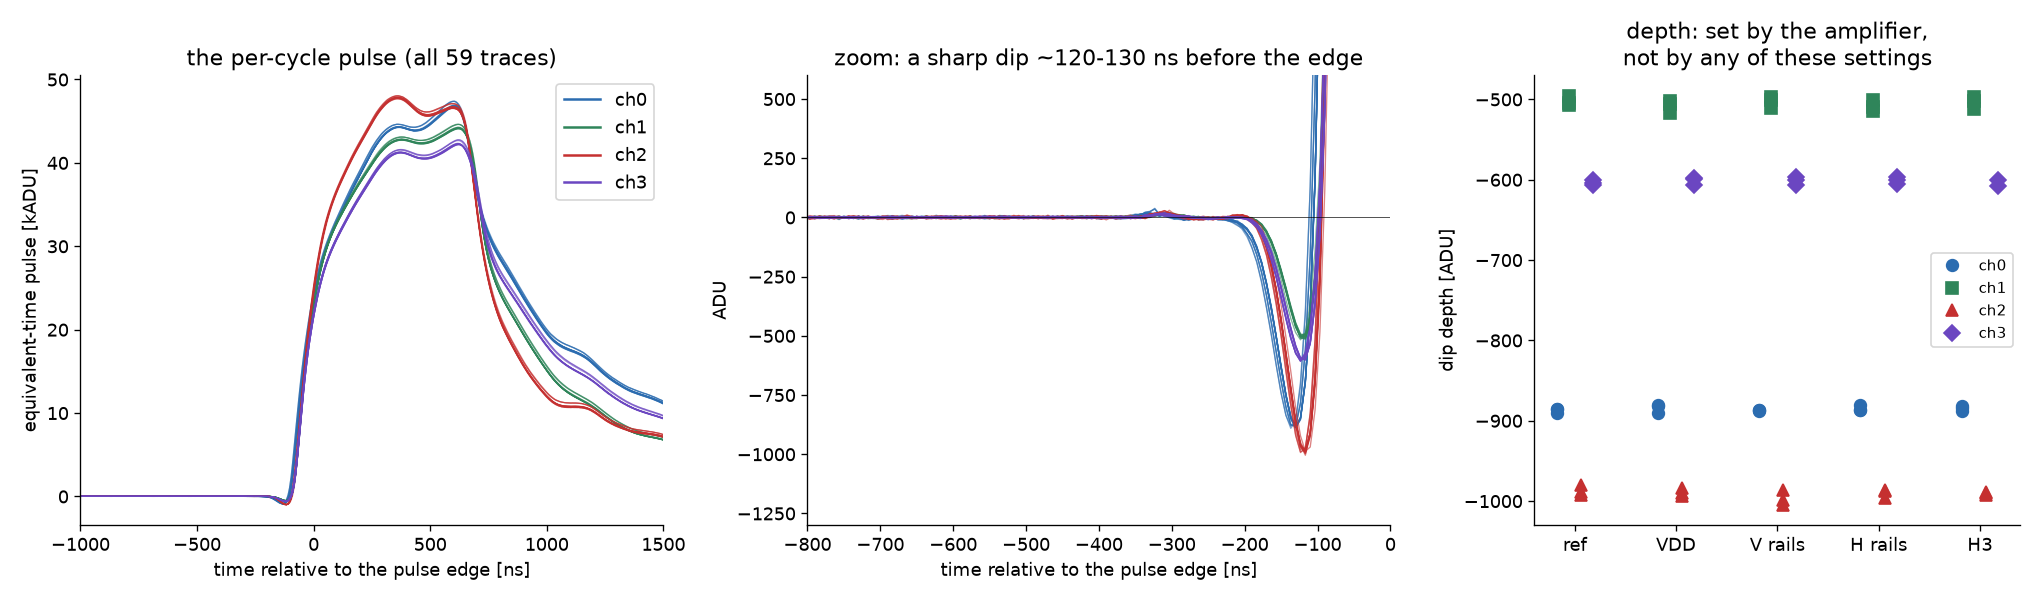
\includegraphics[width=\textwidth]{fig_prepulse_dip.png}
\caption{Left: the per-cycle pulse of all 59 traces. Middle: the dip before it. Right: its depth by setting and
amplifier.}
\label{fig:prepulse}
\end{figure}

\begin{table}[H]
\centering\small
\begin{tabular}{lcccccc}
\toprule
 & ch0 & ch1 & ch2 & ch3 & amp.\ $F$ & repeat share \\
\midrule
dip depth (ADU) & $-886$ & $-505$ & $-990$ & $-601$ & 5851 & 0.001 \\
dip / pulse height & $-0.019$ & $-0.011$ & $-0.021$ & $-0.014$ & 4023 & 0.001 \\
\bottomrule
\end{tabular}
\caption{The pre-pulse dip on the 59 traces (medians). Settings $F$ is 0.2--0.4: none of these settings moved it.}
\end{table}

\paragraph{What it is.} It is not the edge of the pulse itself: the dip/pulse ratio differs by amplifier, and within an
amplifier the dip does not follow the pulse height. In the \code{ReadoutCDS} recipe of \code{reference\_v5.seq}, SW goes
high and RG low together right after the signal window, SW and OG go low 3 units later, then OG and RG go high again.
The dip is most likely the feedthrough of one of the first edges, but the trace flags do not record these clocks. The
session-B packets that move RG\_H, RG\_L and SW\_L by $\pm0.5$\,V will show which rail it follows; then it measures how
strongly that clock couples into each amplifier's output.

%======================================================================
\section{The tier structure}
\label{sec:tiers}

Every trace is reduced to all 141 scalars and 18 curves once, in processing, and all of them are stored. What changes is
which features each model sees. Three layers decide that.

\paragraph{Layer 1: implementation tier} (\code{FEATURES[name].tier}): 0 = the original 85 features, 1 = implement-first
additions (physics-motivated, piloted; 29), 2 = candidate additions (27).

\paragraph{Layer 2: evidence tier} (\code{lvl1/feature\_study.py}, stored in \code{lvl1/feature\_study/evidence\_tiers.json}).
It needs no labels.
\begin{itemize}
  \item \textbf{P, protected} (guard a, adopted): eight direct physical estimators of the labels, chosen by physics and
        given to \emph{every} model, besides their evidence tier. For $\se$: CDS rms (detrended), white noise per skip,
        jump-robust sigma, null-CDS noise, Allan deviation at $n = 50$. For the gain: reset-level scatter (kTC noise),
        pulse per volt RG, dip per volt SW. No direct $\lambda$ estimator exists in a trace yet.
  \item \textbf{A, core:} informative (settings $F$ min $> 10$ or amplifier $F > 10$), repeat share $< 0.5$, at most
        20\,\% NaN, and the most informative member of its redundancy cluster (features with $|\rho_{\rm Spearman}| > 0.95$
        form a cluster). A is split by informativeness into \textbf{A1} (the more informative half) and \textbf{A2}, so
        that all tiers have similar sizes.
  \item \textbf{B, supporting:} informative but redundant, or moderately informative ($F$ 4--10).
  \item \textbf{C, store only:} not informative on the data so far, unstable, mostly NaN, or constant.
\end{itemize}

\begin{table}[H]
\centering\small
\begin{tabular}{lccccc}
\toprule
implementation tier & A1 & A2 & B & C & total \\
\midrule
0 (original) & 27 & 19 & 22 & 17 & 85 \\
1 (new) & 8 & 8 & 4 & 9 & 29 \\
2 (new) & 2 & 9 & 7 & 9 & 27 \\
\midrule
total & 37 & 36 & 33 & 35 & 141 \\
\bottomrule
\end{tabular}
\caption{Evidence tiers by implementation tier.}
\end{table}

\paragraph{Caveat: label-free tiers can demote the best noise estimators.} The evidence tiers reward features that
separate settings or amplifiers, and they pick a cluster's representative by that separation. On these 59 traces the
amplifier dominates every correlation, so ``redundant'' means ``identifies the same amplifier''. As a result the most
direct $\se$ estimator, \code{skip: CDS rms (detrended)}, is in tier B, represented by the number of waveform modes; the
reset-level scatter (kTC noise, the top learned feature on synthetic data) is in B because it hardly separates the
amplifiers. A model restricted to tier A would not see them; that is why P exists. Two further guards were prototyped and not adopted
(Section~\ref{sec:guards}).

The evidence tiers are provisional. They rest on 59 traces at five settings that did not change the noise, so the noise
features were judged by amplifier separation alone.

\paragraph{Layer 3: model feature sets.} These come from the tolerance test (Section~\ref{sec:tolerance}) and are the
defaults of \code{--feature-tiers auto} (\code{MODEL\_TIERS} in \code{lvl1/train\_lvl1.py}): P only for the plain
\code{gp} and \code{gp\_saas}, P + A1 for \code{gp\_dim} (the feature ladder, Section~\ref{sec:ladder}); P + A for \code{nn} and \code{ridge}; everything for \code{trees}; settings only for the \code{settings} and
\code{mean} baselines; P + A + B for all other models. They are starting points: the ladder on real data decides.

%======================================================================
\section{Synthetic tolerance test: how many extra columns can each model take?}
\label{sec:tolerance}

\code{lvl1/feature\_tolerance.py} added 20, 50 or 100 extra columns to the own-trace and reference features of three
synthetic 41-packet datasets (the synthetic world has 17 trace features). Three kinds were tried: independent noise,
near-copies of existing features, and real 2026-10-12 feature values drawn at random (realistic distributions and
outliers, but no information). Every model ran with \code{--quick}.

\begin{figure}[H]
\centering
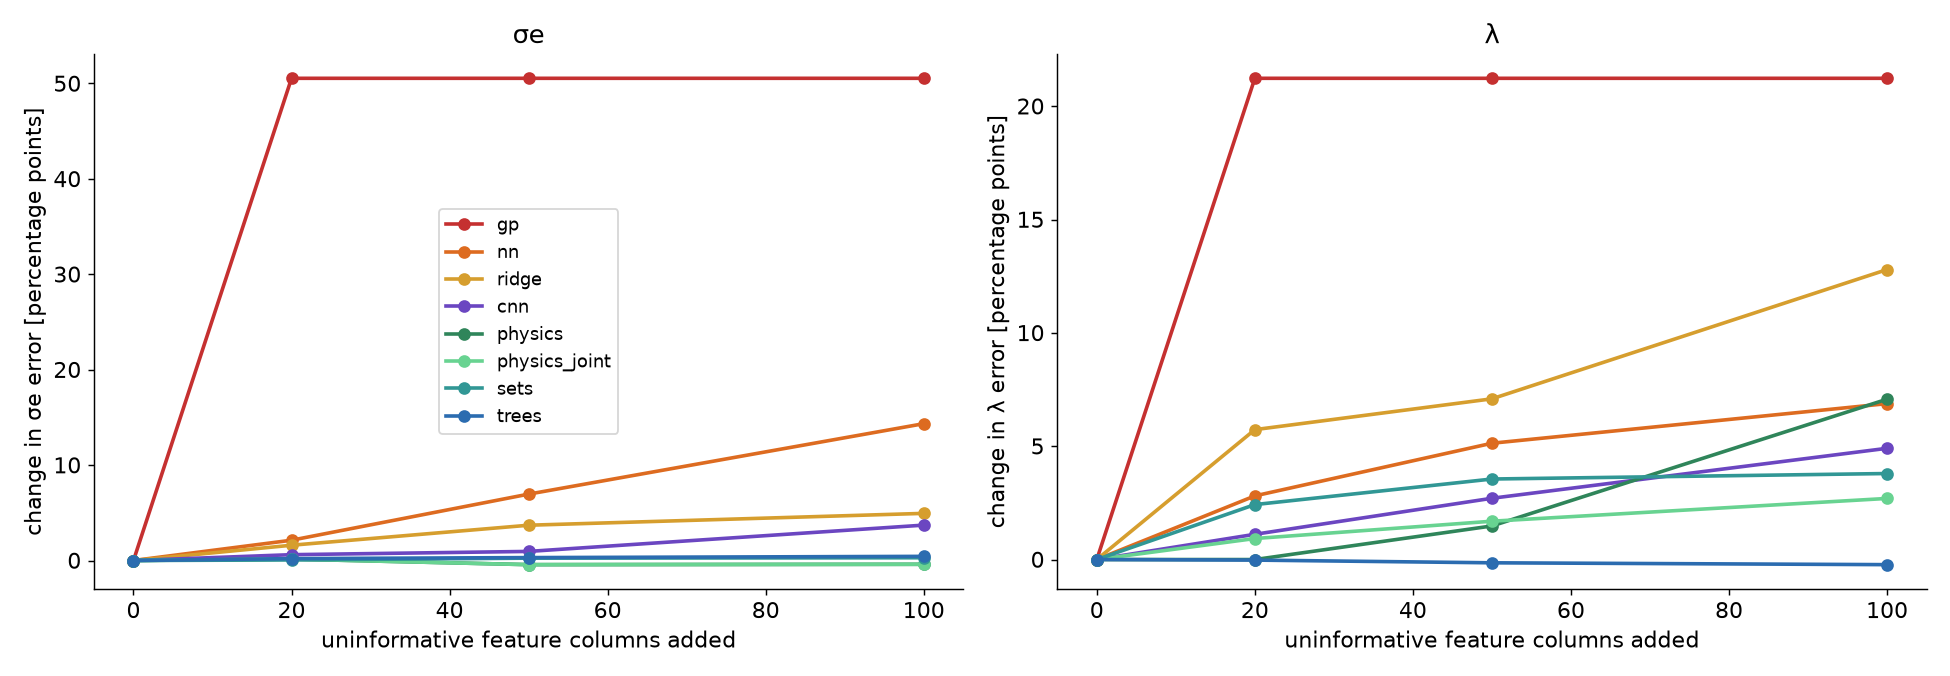
\includegraphics[width=\textwidth]{fig_tolerance.png}
\caption{Change in the error of $\se$ (left) and $\lambda$ (right) as uninformative columns are added (mean of the noise
and real-value kinds, three datasets).}
\label{fig:tol}
\end{figure}

\begin{table}[H]
\centering\small
\begin{tabular}{lcccl}
\toprule
model & base error (\%) & $\Delta\se$ & $\Delta\lambda$ & feature set \\
 & $\se$ / $\lambda$ / gain & +20 / +50 / +100 & +20 / +50 / +100 & \\
\midrule
gp (plain ARD) & 6.9 / 8.0 / 0.9 & \textbf{+51 / +51 / +51} & \textbf{+21 / +21 / +21} & P \\
nn & 10.0 / 17.0 / 1.5 & +2 / +7 / +15 & +3 / +5 / +8 & P + A \\
ridge & 9.5 / 12.4 / 0.9 & +2 / +4 / +5 & +6 / +8 / +14 & P + A \\
cnn & 9.5 / 14.5 / 3.3 & 0 / +1 / +4 & +1 / +3 / +5 & P + A + B \\
physics & 9.1 / 7.4 / 0.9 & 0 / 0 / 0 & 0 / +2.5 / +7 & P + A + B \\
physics\_joint & 9.1 / 4.6 / 0.9 & 0 / 0 / 0 & +1 / +2 / +3 & P + A + B \\
sets & 5.7 / 10.9 / 0.9 & 0 / 0 / 0 & +2.5 / +3.5 / +4 & P + A + B \\
trees & 9.7 / 21.0 / 1.3 & 0 / 0 / 0 & 0 / 0 / 0 & everything \\
\bottomrule
\end{tabular}
\caption{Tolerance test, independent-noise columns ($\Delta$ in percentage points; the real-value columns give the same
within 1--2 points). The gain changes are small except for gp (+30 at +100) and nn (+11). The last column is the
current default (\code{MODEL\_TIERS}); P is the protected set (Section~\ref{sec:tiers}).}
\end{table}

The plain GP collapses to about ``guess the average'' with only 20 uninformative columns. On real data it would see
141 + 141 features, so it gets the protected set P only (the feature ladder, Section~\ref{sec:ladder}). Near-copies hurt much less than uninformative columns, except for the
$\lambda$ of the plain GP (+6 to +11) and of physics (+3 to +5).

%======================================================================
\section{Learned tiers: can a trained model say which features matter?}
\label{sec:learned}

The evidence tiers need no labels. Once there are labels, trained models can rank the features too
(\code{lvl1/feature\_importance.py}). Two independent methods are used for every target (log $\se$, log $\lambda$,
log gain), always with packet-grouped resampling so that a feature is not judged on the rows it was fitted to:

\begin{itemize}
  \item \textbf{Stability selection} \cite{mb2010}: an elastic net (\code{l1\_ratio} 0.5, $\alpha$ from cross-validation)
        is refitted on 30 packet-bootstrap resamples; the importance is how often the feature's coefficient is non-zero.
  \item \textbf{Permutation importance} \cite{breiman2001}: gradient-boosted trees are fitted on four fifths of the
        packets; the importance is how much the held-out squared error grows when the feature is shuffled.
\end{itemize}

\paragraph{Why shadow features.} Ranking the features against each other does not work at this data size. On synthetic
41-packet data, beyond the one or two features that identify the amplifier, real and pure-noise features had the same
importances (about $10^{-4}$). So every column gets a \emph{shadow}: a copy with its rows shuffled, which keeps the
distribution and removes the information (Boruta \cite{boruta2010}). A feature wins a round if its importance exceeds
the 95th percentile of the shadows' importances. There are 5 rounds with fresh shadows; a feature is confirmed by a
method if it wins most of them.

\paragraph{The learned tiers.}
\begin{itemize}
  \item \textbf{L1, confirmed:} both methods confirm the feature, each by more than $1.5\times$ the shadows' 95th
        percentile, for at least one target.
  \item \textbf{L2, candidate:} one method confirms it, or both but narrowly.
  \item \textbf{L3, not shown to matter.}
\end{itemize}

\paragraph{Check on synthetic data.} 20 pure-noise columns (``null 0''--``null 19'') were added to each dataset. A good
rule puts none of them in L1.

\begin{table}[H]
\centering\small
\begin{tabular}{lcccc}
\toprule
dataset & noise in L1, no margin & noise in L1, margin 1.5 & noise in L2 & real features in L1 \\
\midrule
td41\_s0 & 0 & 0 & 6 & 5 \\
td41\_s1 & 0 & 0 & 5 & 4 \\
td41\_s2 & 2 & 0 & 5 & 8 \\
\midrule
td100\_s0 (unseen) & --- & 0 & 3 & 3 \\
td13\_s0 (unseen) & --- & \textbf{1} & 6 & 6 \\
\bottomrule
\end{tabular}
\caption{Learned tiers on synthetic data, 20 noise columns each, rerun on 2026-10-22 with the elastic net's
regularization chosen by packet-grouped folds (row-wise before; ``no margin'' column from the first run). The margin was
chosen on the first three datasets; on the two unseen ones it held at 100 packets but let one noise column into L1 at 13
packets, the size of session A. L1 is therefore a diagnostic, not a guarantee.}
\end{table}

\begin{figure}[H]
\centering
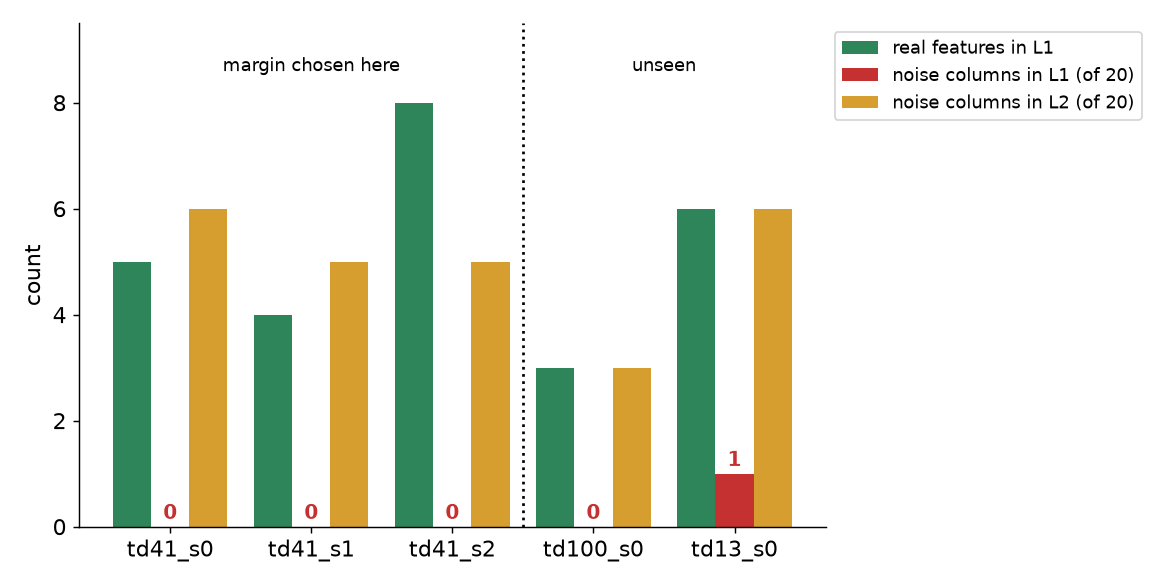
\includegraphics[width=0.8\textwidth]{fig_learned_tiers.png}
\caption{Real features and noise columns per learned tier (grouped-CV rerun): 1 of 100 noise columns reached L1, on the
13-packet dataset.}
\label{fig:learned}
\end{figure}

\paragraph{What it found.} The same features reached L1 in most datasets: the detrended CDS rms and the reset-level
scatter (in all five), the dip recovery time (in four), and the horizontal minimum or maximum (in four). In the synthetic
world the CDS rms is $\sigma_1 \times$ gain and the reset-level scatter follows $\sigma_1$, so these two carry $\se$ and
the gain directly; the horizontal levels follow the H low rails, which drive the clock-induced charge and so $\lambda$.
The method finds what is really there. One feature that responds to no setting, the within-cycle power at 1--3\,MHz,
reached L1 once (td41\_s2). It is not a false positive: every synthetic amplifier has its own offset of each feature, so
this feature identifies the amplifier, and the amplifier carries information about $\se$.

\paragraph{What this means.} L1 can be used as a feature set. L2 cannot: 4--8 of 20 noise columns (20--40\,\%) reached
it, so it is only a list of features worth a look. The caveat is that the margin was tuned on three of the five
datasets; the two unseen ones agree, but this is still synthetic data.

\paragraph{Use on real data.} After session A, run it beside the evidence study as a \emph{diagnostic}: features in L1
but not in tier A, and tier-A features in L3, are the ones to look at physically. It does not choose any model's
features (Section~\ref{sec:guards}).

%======================================================================
\section{Training with tiers}
\label{sec:tooling}

\code{lvl1/train\_lvl1.py} has these options for the feature sets:

\begin{itemize}
  \item \code{--feature-tiers SPEC}: \code{all}, \code{none} (settings only), \code{auto} (the per-model defaults of
        Section~\ref{sec:tiers}), or tier labels joined by \code{+}, e.g.\ \code{P+A}, \code{A1}, \code{impl0}. It
        selects the matching columns of both the own-trace and the reference features.
  \item \code{--tier-ablation [SET ...]}: train every model on every set (default \code{none P P+A1 P+A P+A+B all impl0})
        and compare each, paired over packets, with the same model on \code{--ablation-ref} (default \code{all}).
  \item \code{--feature-ladder [ORDER ...]}: feed every model more and more features in \emph{label-free} orders and
        report error against the number of features (Section~\ref{sec:ladder}).
  \item \code{--tier-file}: another evidence-tier file, e.g.\ the one finalized on session A.
\end{itemize}

\subsection{Guards against the label-free tiers}
\label{sec:guards}

The evidence tiers measure separation, not prediction. Four guards were prototyped and tested on synthetic data: the
three synthetic 41-packet datasets, plus the 120 other real features as uninformative columns with their real names
(values drawn at random), so that the tiers act as they would on real data.

\begin{table}[H]
\centering\small
\begin{tabularx}{\textwidth}{Lccc}
\toprule
feature set & gp & nn & ridge \\
\midrule
A (the old default) & collapsed & 32.9 / 22.4 / 17.6 & 16.8 / 19.9 / 4.4 \\
(a)--(c): P + tiers with within-amplifier clusters and no repeat penalty & collapsed & 21.7 / 21.9 / 10.2 & 14.7 / 23.2 / 3.3 \\
(a) alone: P & 9.6 / 22.0 / 0.9 & 12.9 / 18.6 / 6.3 & 12.2 / 17.0 / 6.3 \\
(a) + (d): P + a set chosen with labels on other datasets & 9.0 / 14.5 / 0.9 & 10.2 / 16.9 / 2.6 & 9.5 / 14.0 / 0.9 \\
the 17 true synthetic features & 6.9 / 8.0 / 0.9 & 10.1 / 17.1 / 1.5 & 9.5 / 12.4 / 0.9 \\
\bottomrule
\end{tabularx}
\caption{Error \% ($\se$ / $\lambda$ / gain), mean of three datasets, short training. ``Collapsed'' = no better than the
training mean.}
\end{table}

\textbf{Adopted: (a), the protected tier P.} \textbf{Not adopted:} (b) clusters within each amplifier and (c) no repeat
penalty, which helped less and enlarge tier A; and (d) choosing features by the labels. (d) nearly reaches the true
features here, but its ranking came from sibling datasets of a known world, the optimistic case. On $\sim$30 real
packets a ranking by the labels is noisy (the winner's curse), optimistic unless redone inside every fold, favours the
settings scanned so far, and lets the labels' own errors steer the choice. The labels therefore score a few fixed sets
but never order the features.

\subsection{The feature ladder}
\label{sec:ladder}

Every model is trained on a nested series of feature sets on the same folds, and its error is read against the number
of features. None of the orders uses the labels, so they can be frozen before the first labels are seen.

\begin{table}[H]
\centering\small
\begin{tabularx}{\textwidth}{>{\raggedright\arraybackslash}p{1.4cm}>{\raggedright\arraybackslash}p{5.2cm}L}
\toprule
order & steps & what it asks \\
\midrule
\code{tiers} & none $\to$ P $\to$ P+A1 $\to$ P+A $\to$ P+A+B $\to$ all & does each evidence tier help this model? \\
\code{cover} & P $\to$ 15 $\to$ 25 $\to$ 40 $\to$ 60 $\to$ 90 $\to$ all & the next feature is the one least explained by those
already taken (column-pivoted QR of the standardized features, after P): even coverage, no preference for amplifier separation \\
\code{random} & P, then the same sizes in 3 random orders & the control: does the order matter at all? \\
\code{groups} & P + one physics group at a time & which family adds what (not nested) \\
\bottomrule
\end{tabularx}
\caption{The label-free orders of \code{--feature-ladder}.}
\end{table}

The report gives error per step, the paired difference against the same model on P, a plot, and a suggested set per
model and target: the smallest step within one standard error of the model's best step.

\begin{figure}[H]
\centering
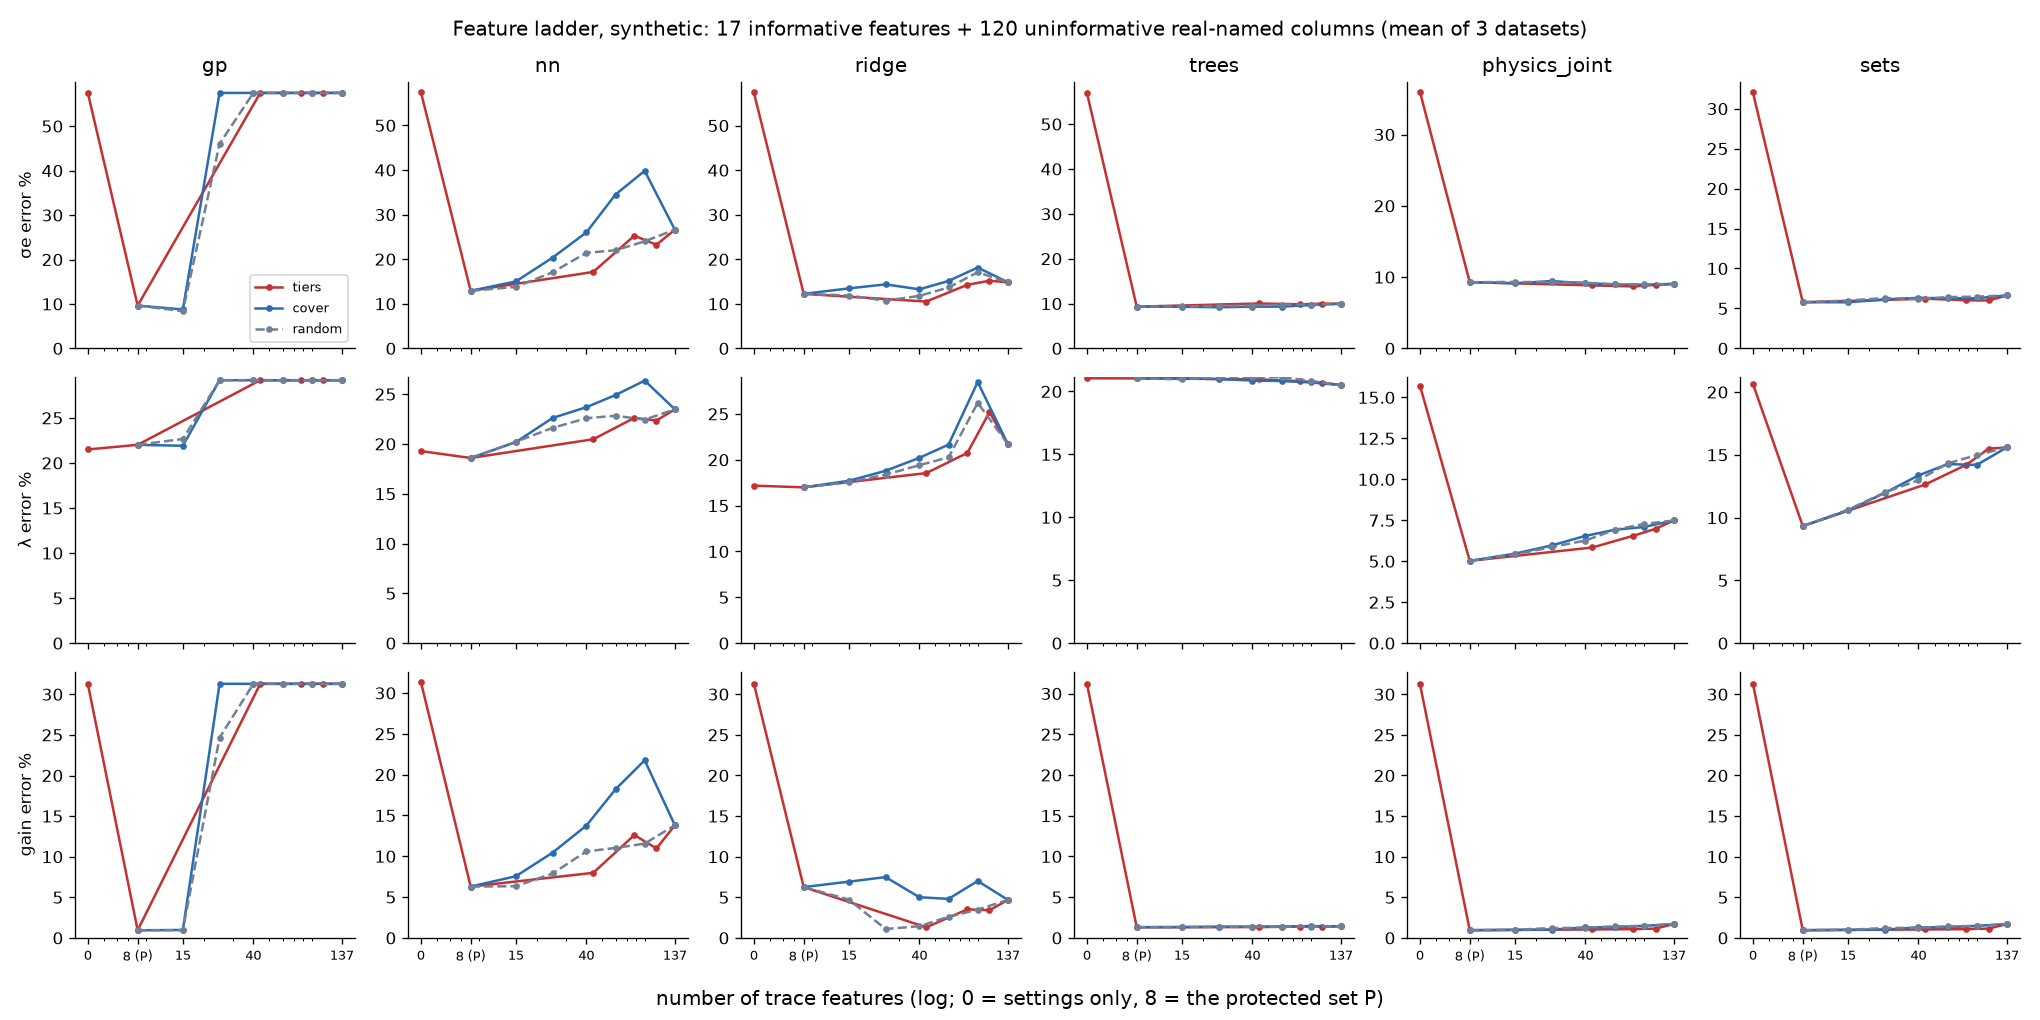
\includegraphics[width=\textwidth]{fig_feature_ladder.png}
\caption{The ladder on synthetic data (17 informative features + 120 uninformative real-named columns; mean of three
datasets; short training).}
\label{fig:ladder}
\end{figure}

On this all-junk test (Figure~\ref{fig:ladder}): the plain GP is best at 8--15 features and collapses beyond 15--25 in
every order, so its default is now P only; \code{gp\_dim} stays flat up to all 137 features (its dimension-scaled prior
prevents the collapse; best $\se$ 8.4\,\% at P + A1, its default); \code{gp\_saas} keeps $\se$ and the gain but its
$\lambda$ gets worse with every step (19\,\% at P, 30\,\% with all), so its default is P; nn gets steadily worse with every step; ridge is best around 25--45 features;
trees are flat; physics\_joint and sets are flat for $\se$ and the gain but lose on $\lambda$ as features are added
(sets 9.3\,\% at P, 15.6\,\% with all). The cover order did not beat the random control, as expected: without labels no
order can know which of these columns carry information. On real data, where many A and B features carry information,
comparing the orders is the point.

%======================================================================
\section{Plan for the first real data}
\label{sec:plan}

\begin{enumerate}
  \item \textbf{Freeze the ladder before the first labels.} The orders (\code{tiers}, \code{cover}, \code{random},
        \code{groups}) use the features only; fix them, and the steps, before session A's labels are seen.
  \item \textbf{Update the tiers after session A, without labels.} Rerun \code{lvl1/feature\_study.py} on the real
        packets: the delayInt packets are the first where noise features can separate settings. Label relevance and the
        learned tiers (\code{lvl1/feature\_importance.py}) are reported beside the tiers as diagnostics, not used to move
        features. A feature joins P only with a stated physical mechanism. Revise once more after session B; never use
        session C for this.
  \item \textbf{Run the ladder for every model} (\code{--feature-ladder tiers cover random groups}) on sessions A + B,
        with the setting-grouped folds. Read each model's curve; take the smallest step within one standard error of
        its best.
  \item \textbf{Confirm once on session C} (\code{--holdout-session C}), report every step of every order, and keep the
        number of steps fixed in advance: picking the best of many on about 30 packets is optimistic \cite{cawley2010}.
\end{enumerate}

\paragraph{Open items.} Label relevance as a reported column of \code{feature\_study.py}; the ladder on real data.

%======================================================================
\section{Files}

\begin{table}[H]
\centering\small
\begin{tabularx}{\textwidth}{>{\raggedright\arraybackslash}p{6.2cm}L}
\toprule
file & what \\
\midrule
\code{src/trace\_features\_extra.py} & the 56 new features (including the \code{clock:} group and the pre-pulse dip) and 4 curves \\
\code{lvl1/feature\_study/prepulse\_pilot/} & the pre-pulse dip pilot (script, numbers, figure) \\
\code{lvl1/feature\_study/clock\_pilot/} & the clocking-region pilot (script, numbers, figure) \\
\code{lvl1/feature\_study/ladder\_synthetic/} & the synthetic feature-ladder results and figure \\
\code{src/trace\_features.py} & the \code{tier} attribute and \code{names\_by\_tier()} \\
\code{tests/test\_trace\_features\_new.py} & 19 tests with known answers \\
\code{lvl1/feature\_study.py} & evidence tiers; results in \code{lvl1/feature\_study/README.md} \\
\code{lvl1/feature\_tolerance.py} & the synthetic tolerance test \\
\code{lvl1/feature\_importance.py} & learned tiers L1/L2/L3 \\
\code{lvl1/train\_lvl1.py} & \code{--feature-tiers}, \code{--tier-ablation}, \code{--feature-ladder} \\
\code{lvl1/new\_trace\_features.ipynb} & walkthrough notebook of the new features \\
\code{docs/trace\_features\_and\_tiers.md} & the working document behind this note \\
\code{make\_figures.py} (in this folder) & the figures of this note \\
\bottomrule
\end{tabularx}
\end{table}

%======================================================================
\begin{thebibliography}{99}
\bibitem{ads2012} T.~G. Andersen, D.~Dobrev, E.~Schaumburg, Jump-robust volatility estimation using nearest neighbor
  truncation, \emph{J. Econometrics} 169 (2012) 75--93.
\bibitem{lm2008} S.~S. Lee, P.~A. Mykland, Jumps in financial markets: a new nonparametric test and jump dynamics,
  \emph{Rev. Financial Studies} 21 (2008) 2535.
\bibitem{bns2004} O.~E. Barndorff-Nielsen, N.~Shephard, Power and bipower variation with stochastic volatility and jumps,
  \emph{J. Financial Econometrics} 2 (2004) 1--37.
\bibitem{thomson1982} D.~J. Thomson, Spectrum estimation and harmonic analysis, \emph{Proc. IEEE} 70 (1982) 1055--1096.
\bibitem{riley2008} W.~J. Riley, \emph{Handbook of Frequency Stability Analysis}, NIST Special Publication 1065 (2008).
\bibitem{hua1990} Y.~Hua, T.~K. Sarkar, Matrix pencil method for estimating parameters of exponentially damped/undamped
  sinusoids in noise, \emph{IEEE Trans. ASSP} 38 (1990) 814--824.
\bibitem{richman2000} J.~S. Richman, J.~R. Moorman, Physiological time-series analysis using approximate entropy and
  sample entropy, \emph{Am. J. Physiol. Heart Circ. Physiol.} 278 (2000) H2039--H2049.
\bibitem{allen1978} R.~Allen, Automatic earthquake recognition and timing from single traces, \emph{Bull. Seismol. Soc.
  Am.} 68 (1978) 1521--1532.
\bibitem{ligo2020} LIGO Scientific Collaboration and Virgo Collaboration, A guide to LIGO--Virgo detector noise and
  extraction of transient gravitational-wave signals, \emph{Class. Quantum Grav.} 37 (2020) 055002.
\bibitem{randall2011} R.~B. Randall, J.~Antoni, Rolling element bearing diagnostics: a tutorial, \emph{Mech. Syst. Signal
  Process.} 25 (2011) 485--520.
\bibitem{wang2006} X.~Wang, P.~R. Rao, A.~Mierop, A.~J.~P. Theuwissen, Random telegraph signal in CMOS image sensor
  pixels, \emph{IEEE IEDM} (2006) 115--118.
\bibitem{boruta2010} M.~B. Kursa, W.~R. Rudnicki, Feature selection with the Boruta package, \emph{J. Stat. Software} 36
  (2010) 1--13.
\bibitem{mb2010} N.~Meinshausen, P.~B\"uhlmann, Stability selection, \emph{J. R. Stat. Soc. B} 72 (2010) 417--473.
\bibitem{breiman2001} L.~Breiman, Random forests, \emph{Machine Learning} 45 (2001) 5--32.
\bibitem{cawley2010} G.~C. Cawley, N.~L.~C. Talbot, On over-fitting in model selection and subsequent selection bias in
  performance evaluation, \emph{J. Mach. Learn. Res.} 11 (2010) 2079--2107.
\end{thebibliography}

\end{document}
